\section{Sesión 8}

\begin{teorema}
	Suponga que $g:I\to\mathbb{R}$ es diferenciable y que $g'$ es integrable en $I$. Sea $g(I)=J$. Si $f:J\to\mathbb{R}$ es continua, entonces, $\forall a,b \in I$, se cumple: 
	$$\int_a^b f(g(x))g'(x)dx=\int_{g(a)}^{g(b)}f(u)du,$$
\end{teorema}


\begin{prop}
	Suponga que $f_n:[a,b]\to\mathbb{R}$, donde $n\in \mathbb{Z}^+$ y $f_n\in R[a,b], \forall n$; y suponga que $f_n \longrightarrow_{uniforme} f$ sobre $[a,b]$. Entonces: 
	\begin{enumerate}
		\item $f\in R[a,b]$. 
		\item $\lim_{n\to\infty}\int_a^b f_n=\int_a^b f$.
		\end{enumerate} 
\end{prop}

\subsection{Integrales impropias}

\begin{definicion}
	Suponga que $f:(a,B]\to\mathbb{R}$ es Riemman integrable en $[c,d]\ni a<c<b$. Entonces, la integral impropia de $f$ sobre $[a,b]$ es: 
	$$\int_a^b f=\lim_{\varepsilon\to 0}\int_{a+\varepsilon}^b f.$$
	La integral impropia converge si este límite existe. En otro caso, la integral diverge. 
\end{definicion}

\begin{definicion}
	Suponga que $f:[a,\infty)\to\mathbb{R}$ es integrable sobre $[a,r], r>a$. Entonces, la integral impropia de $f$ es: 
	$$\int_a^\infty f =\lim_{r\to\infty}\int_a^r f.$$
\end{definicion}

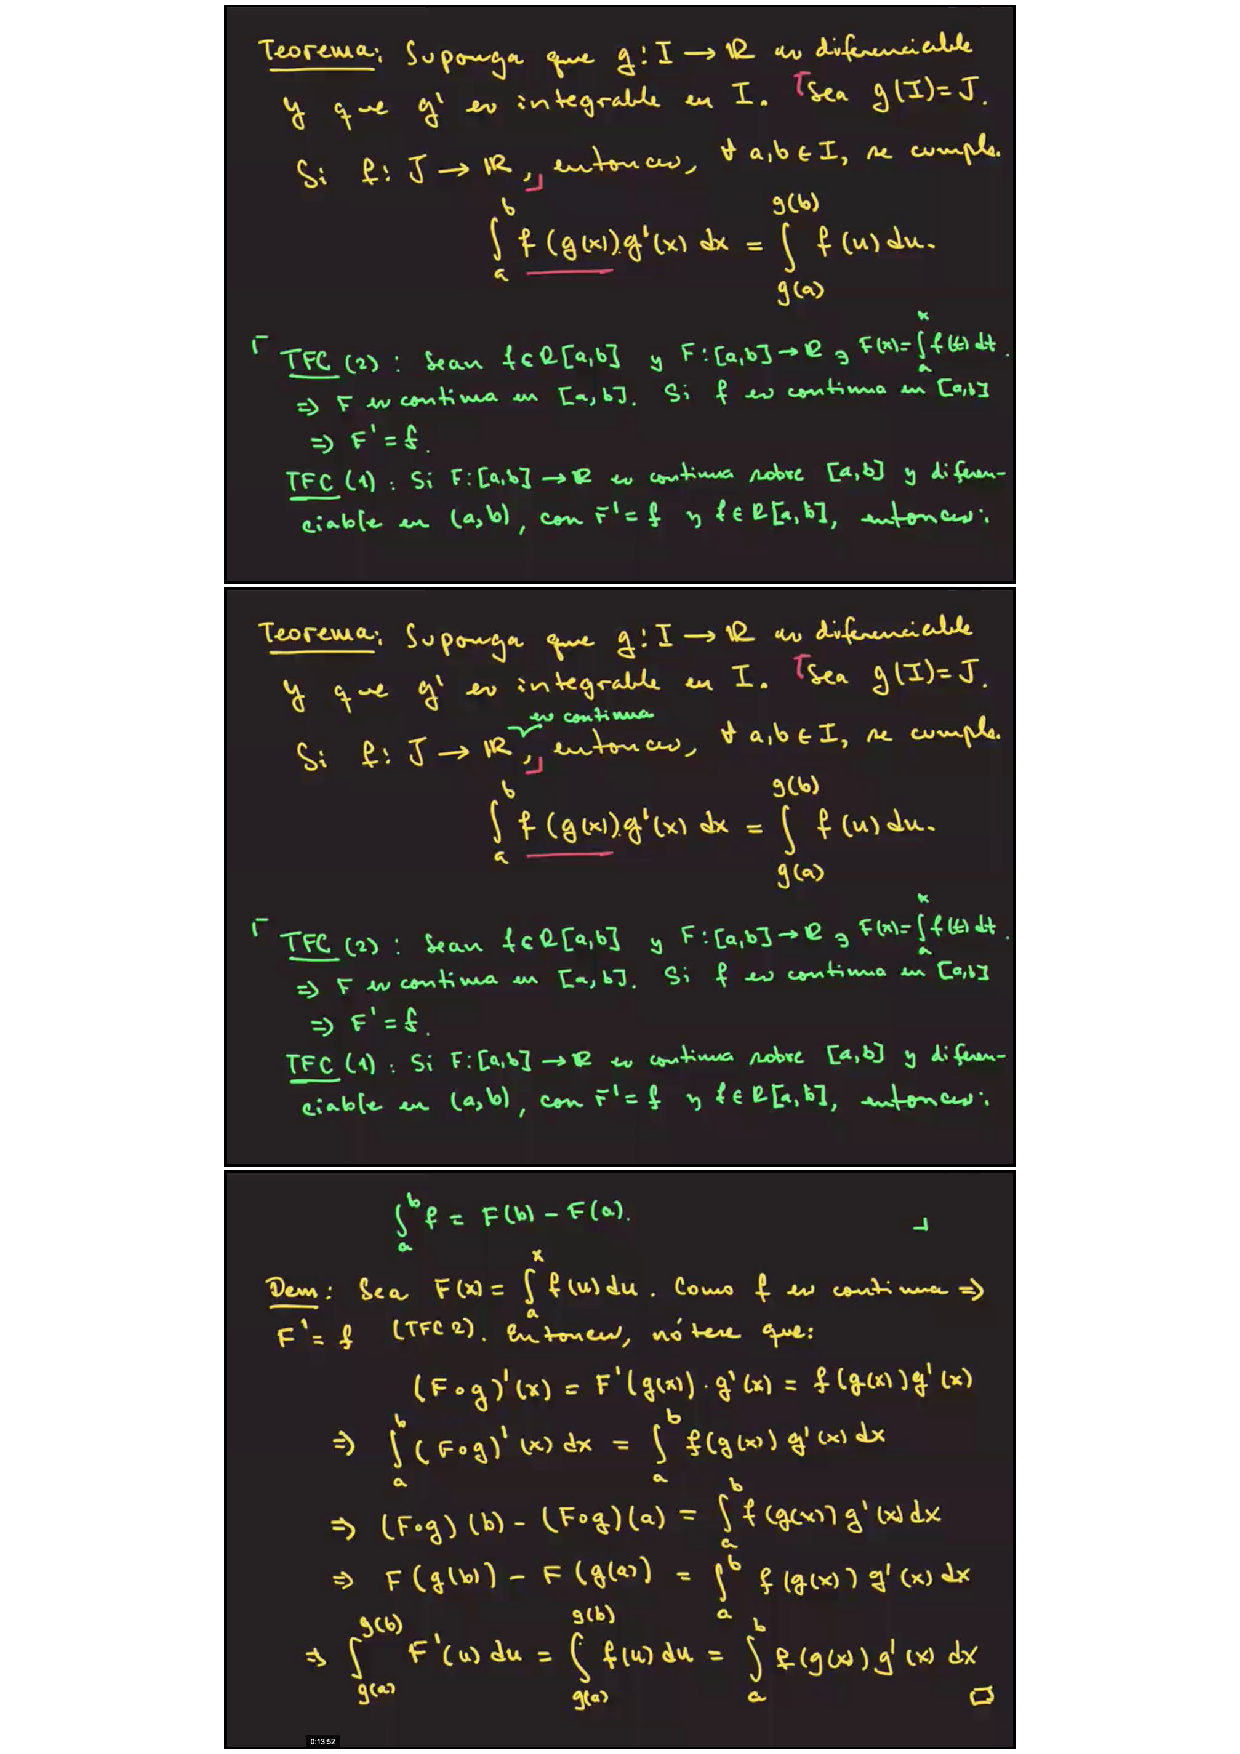
\includepdf[pages=-]{apendices/s8.pdf}